\section{The Central Finding: Ghost-Safe Does Not Mean Vignetting-Safe}

This is the single most important experimental result to come out of the
whole geometry comparison, and it is worth stating plainly before looking
at any numbers: \textbf{a design can have an infinite ghost-safety margin at
straight-ahead gaze (meaning literally no two holes are ever simultaneously
active under the pupil) and still fail the vignetting check once the eye
looks around.}

\intuitbox{Why this makes physical sense: ``no two holes active at once'' at
$\varphi=0$ only describes one single eye position. As the pupil shifts
during rotation, holes that were previously outside its reach can come
into play together, creating an active pair that did not exist before.
Zero risk at one gaze angle says nothing about zero risk at every other
gaze angle --- these genuinely are two separate conditions to check.
}
Figure~\ref{fig:divergence} shows how often this actually happens, measured
directly from the data (not assumed): for every family, the fraction of
straight-ahead-safe designs that turn out to \emph{fail} the vignetting
check ranges from 37.8\% (concentric rings, the most robust family) to
88.9\% (Fibonacci spiral / golden angle, the least robust). This is not a
small-print caveat --- for the spiral families, roughly nine out of ten
designs that look perfectly safe under the simplest possible check turn out
to be unsafe once you account for how eyes actually move.

\begin{figure}[h]
\centering
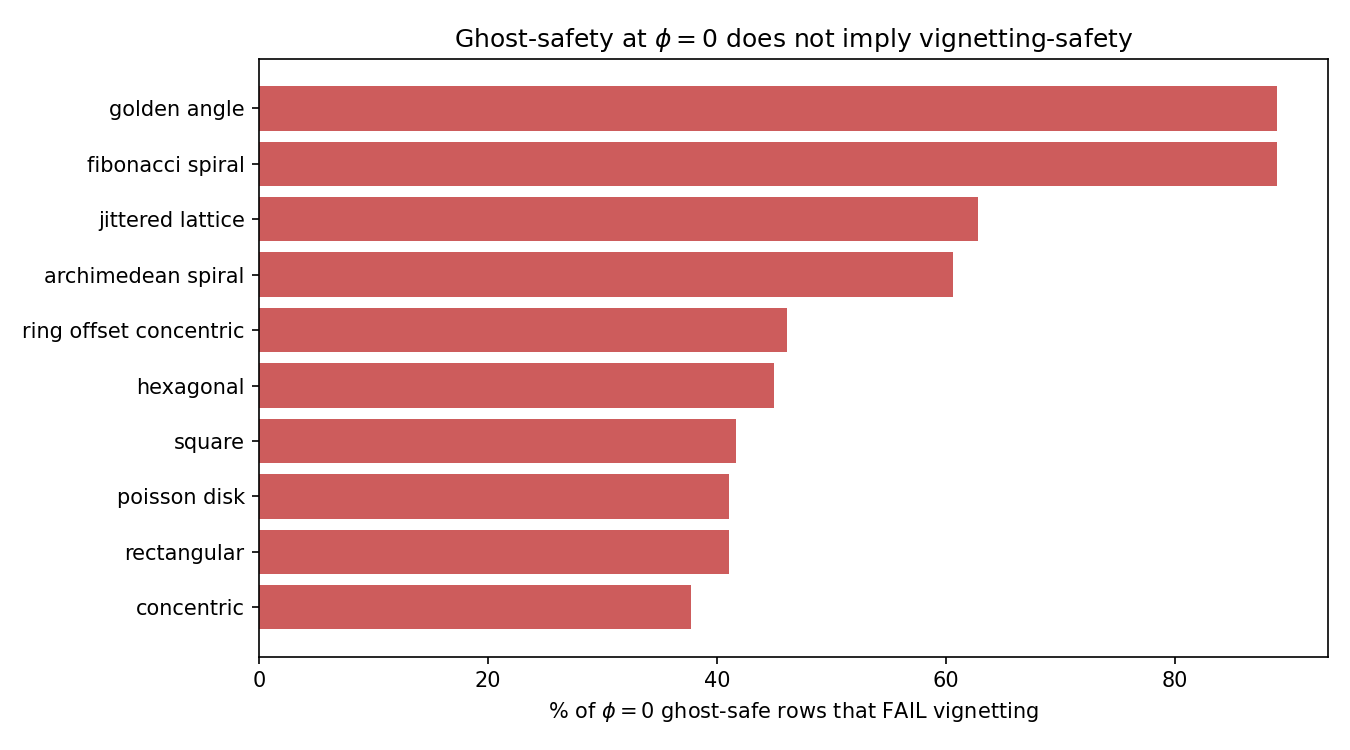
\includegraphics[width=0.85\textwidth]{handbook_figs/fig_divergence.png}
\caption{Fraction of straight-ahead ghost-safe designs, per geometry family,
that fail the vignetting check once gaze angle is properly integrated.}
\label{fig:divergence}
\end{figure}

\codemapbox{This is why \texttt{comparison\_metric/gates.py} applies both gates as
independent, separately-required conditions
(\texttt{apply\_gates()} with both \texttt{gate\_ghost\_safety} and
\texttt{gate\_vignetting\_safety}), rather than treating one as a
shortcut proxy for the other.
}
\section{A Real Bug Worth Understanding: When ``Density'' Stops Making Sense}

\subsection{The Problem}

Packing density --- how many holes fit per unit area --- sounds like a
simple thing to compute: count the holes, divide by the area they occupy.
But ``the area they occupy'' is a genuinely tricky question once a
requested pattern collapses down to very few actual holes (because the
overlap-rejection step, described above, removed most of them).

\intuitbox{Picture a formula that assumes a repeating grid pattern (a ``unit cell''
multiplied by how many times it repeats). If overlap-rejection has reduced
a requested 20-hole pattern down to just \emph{one} surviving hole, there is
no repeating grid left to describe --- the formula's own assumption has
silently stopped applying, but nothing in the code was told to notice. The
formula still returns a number; it is simply a meaningless one.
}
This defect was real and it mattered: it was caught only because a
resulting design's reported density implied that its holes covered
\emph{more area than the space they were packed into} --- a value greater
than 100\% open area, which is a plain physical impossibility and an
excellent kind of bug to have a numerical assertion check for automatically,
rather than relying on a human noticing an oddly large number.

\subsection{The Fix, and the Lesson}

The fix required two separate corrections, because two different families
of geometry broke in two different ways:
\begin{enumerate}
  \item For lattice families (square, hex, rectangular), the fix is a
  \emph{feasibility check}: before trusting a unit-cell-based density, first
  confirm the requested spacing is even geometrically large enough to
  contain one hole. This check depends only on the ratio of hole size to
  spacing --- it is completely independent of how many holes actually
  survived, which is exactly why simply requiring ``at least 4 holes''
  \emph{could not} have caught this case on its own.
  \item For the ring/spiral/random families, the area was originally
  computed from the hole \emph{centers} only, forgetting that each hole
  also has its own physical radius extending past its center --- an
  omission proven with a real 7-hole test case where every hole was
  correctly non-overlapping, yet the naive area still came out too small.
  The fix adds each hole's own radius as a buffer around the boundary
  before computing area (a Minkowski/offset-buffer correction).
\end{enumerate}

The broader lesson, useful well beyond this one bug: \textbf{a formula that
is correct in the typical case can silently become meaningless in an edge
case, and the only reliable way to catch that is to check the answer
against a fact you know must always be true} --- here, that open area can
never exceed 100\%. Guessing at ``reasonable-looking'' thresholds (like a
minimum hole count) is not a substitute for that kind of physical sanity
check.

\codemapbox{The final, corrected logic lives in a single shared file,
\texttt{array\_geometry\_lab/degeneracy\_filter.py}, imported by every
downstream script rather than re-implemented separately in each one --- so
a future new geometry family only has to get this right once.
}
\newpage
